%%%%%%%%%%%%%%%%%%%%%%%%%%%%%%%%%%%%%%%%%%%
%%%%%%%%%%%%%%%%%%%%%%%%%%%%%%%%%%%%%%%%%%%
%%%%%%%%%%%%%%%%%%%%%%%%%%%%%%%%%%%%%%%%%%%
\chapter{State of the Art}
\label{Sec:star}
In this chapter we will present the state of the art work present in bioinformatical literature with regards to the visualization and analysis of proteins and their interactions with other molecules. We will start with overview of existing molecular visualization techniques, then continue with the work related to protein-ligand interactions, where literature covers a substantial amount of diverse research. The end of this chapter will be dedicated to protein-protein interactions. 

\section{Molecular Visualization}
Many different molecular representations have developed to cater for diverse needs of molecular biologists. Although some new representations are still emerging, the research in this area is currently more focused on development of fast visualization algorithms and GPU-based acceleration of traditional ones, in order to represent large and dynamic molecular data. Here we will provide the overview of typical molecular representations and they state of the art execution. There are, however, countless of other approaches that exceed the capacity of this work. The detailed study concerning molecular representation can be found in state of the art report by Kozlikova et al. \cite{kozlikova2015visualization}. Available is also the report by Patané and Spagnuolo focusing on modeling of molecular surfaces \cite{patane2015state}.

\subsection{Atomistic and Bond-Centric Models}
\begin{wrapfigure}{r}{0.33\textwidth} 
\vspace{-65pt}
  \begin{center}
  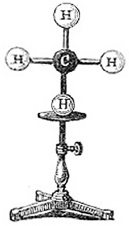
\includegraphics[width=0.65\linewidth]{pictures/04_hoffman.jpg} 
  \caption{Hoffman's methane (Marsh-gas) representation \cite{perkins2005history}.}
  \label{Fig:hoffman}  
\end{center}
  \vspace{-30pt}
\end{wrapfigure}

We can say that history of molecular visualization dates back to the 19th century. In 1808 John Dalton published his atomic theory~\cite{dalton1808new}, where he represented atoms and simple molecules with circular shapes. Couple of decades later, around 1860, August Wilhelm von Hoffmann started using first 3D models of molecules in his lectures at Royal Institution of Great Britain~\cite{perkins2005history} -- see Figure \ref{Fig:hoffman}. This type of molecular representation is called \textit{ball-and-stick} model, where balls represent atoms and sticks represent bonds between them. With couple of modifications this representation is commonly used also nowadays (Figure \ref{Fig:vis} b)). 

Over the years other derivations of ball-and-stick model emerged. In 1959 André Dreiding introduced molecular modelling kit using \textit{stick-only} model~\cite{dreiding1959einfache}. Here the atoms were not represented by balls, but merely as connection points between sticks. Nowadays this model is called also \textit{liquorice} or \textit{Dreiding's model} (Figure \ref{Fig:vis} a)). The colouring of the sticks is often used to indicate atoms or their properties.

Although several researchers, including Dalton and Hoffman, claimed that different atoms have different radii, it wasn't until 1873 that the sizes of atoms were experimentally derived by Johannes Diderik van der Waals~\cite{Waals1873PhDThesis}. In later years this discovery led to so called \textit{space-filling} molecular representations, also called \textit{callote} or \textit{CPK models} after chemists Robert Corey, Linus Pauling, and Walter Koltun \cite{corey1953molecular}. In this representation, full "space-filling" sizes of atoms are used, which provides the overview of molecular surface (Figure \ref{Fig:vis} c)).

\begin{figure}[H]
  \centering
  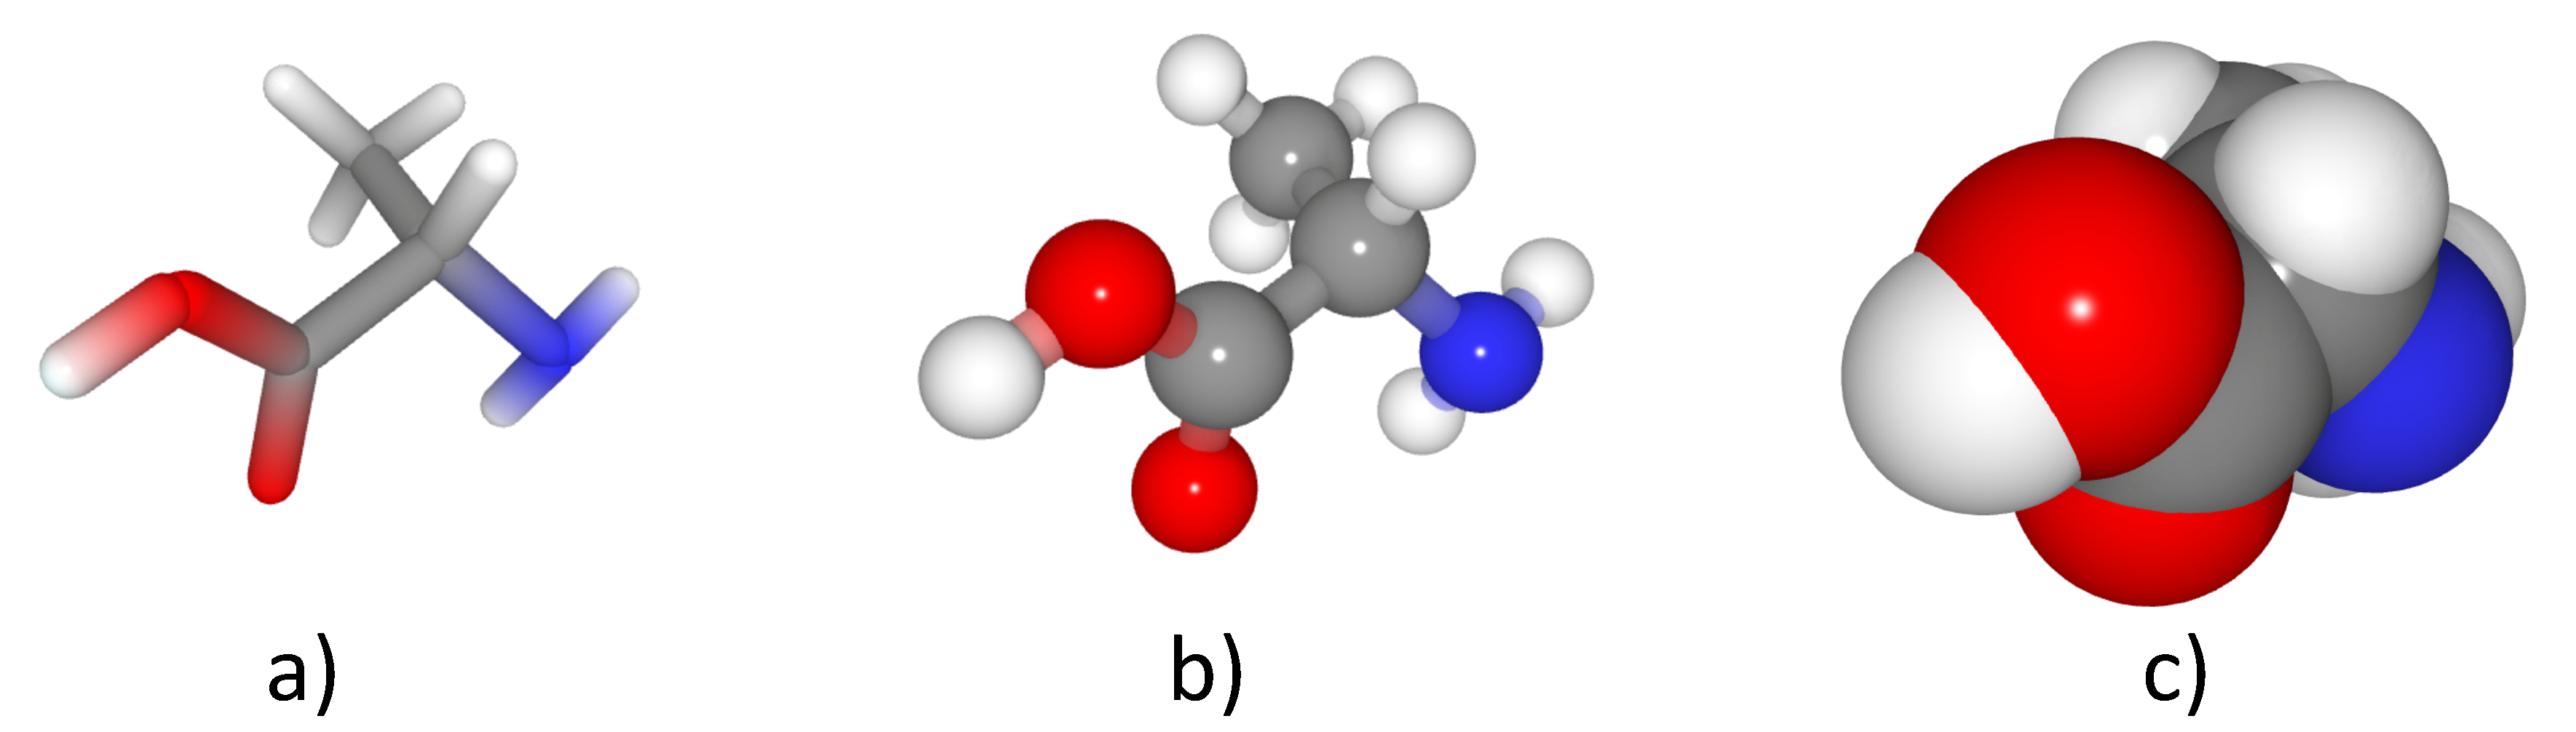
\includegraphics[width=\linewidth]{pictures/vis.pdf} 
  \caption{Types of molecular representations in modern visualization tools: a) liquorice model b) ball-and-stick model c) space-filling model}
  \label{Fig:vis}  
\end{figure} 

Atom and bond based representations of molecules can be decomposed into primitive shapes such as spheres and cylinders, which makes them suitable for GPU-based ray casting. Most of the state of the art rendering techniques stem from glyph ray casting introduce by Gumhold et al. \cite{gumhold2003splatting}, however many performance speedups focusing on rendering of large dynamic molecular structures exist. Since these techniques are focusing on large data samples, they often utilize level of detail (LOD) strategies. Example of this can be the two-level approach of Lampe et al. \cite{lampe2007two} where residues are each residue is represented by one vertex and the atoms in the residues are generated on-the-fly on the GPU. Another approach is used by Le Muzic et al. \cite{le2014illustrative}, where atom positions are stored in a texture and reconstructed using tessellation and geometry shaders.

\subsection{Protein Architecture}
The afore mentioned representations of molecules provide detail information about arrangement of atoms in a molecule. However, for proteins, which can consist of thousands of atoms, this representations can be too cluttered. Therefore, several schematic visualizations were developed.

One of the simplest representations of protein structure is called \textit{alpha trace}. It depicts only the backbone of the protein, as it is derived from the positions of $\alpha$-carbons (Figure \ref{Fig:vis2} a)). This representation provides coarse overview of tertiary and quaternary structure of the protein -- spatial arrangement of the polypeptide chains. However, it can be difficult to identify secondary structures from the alpha trace.

\begin{figure}[H]
  \centering
  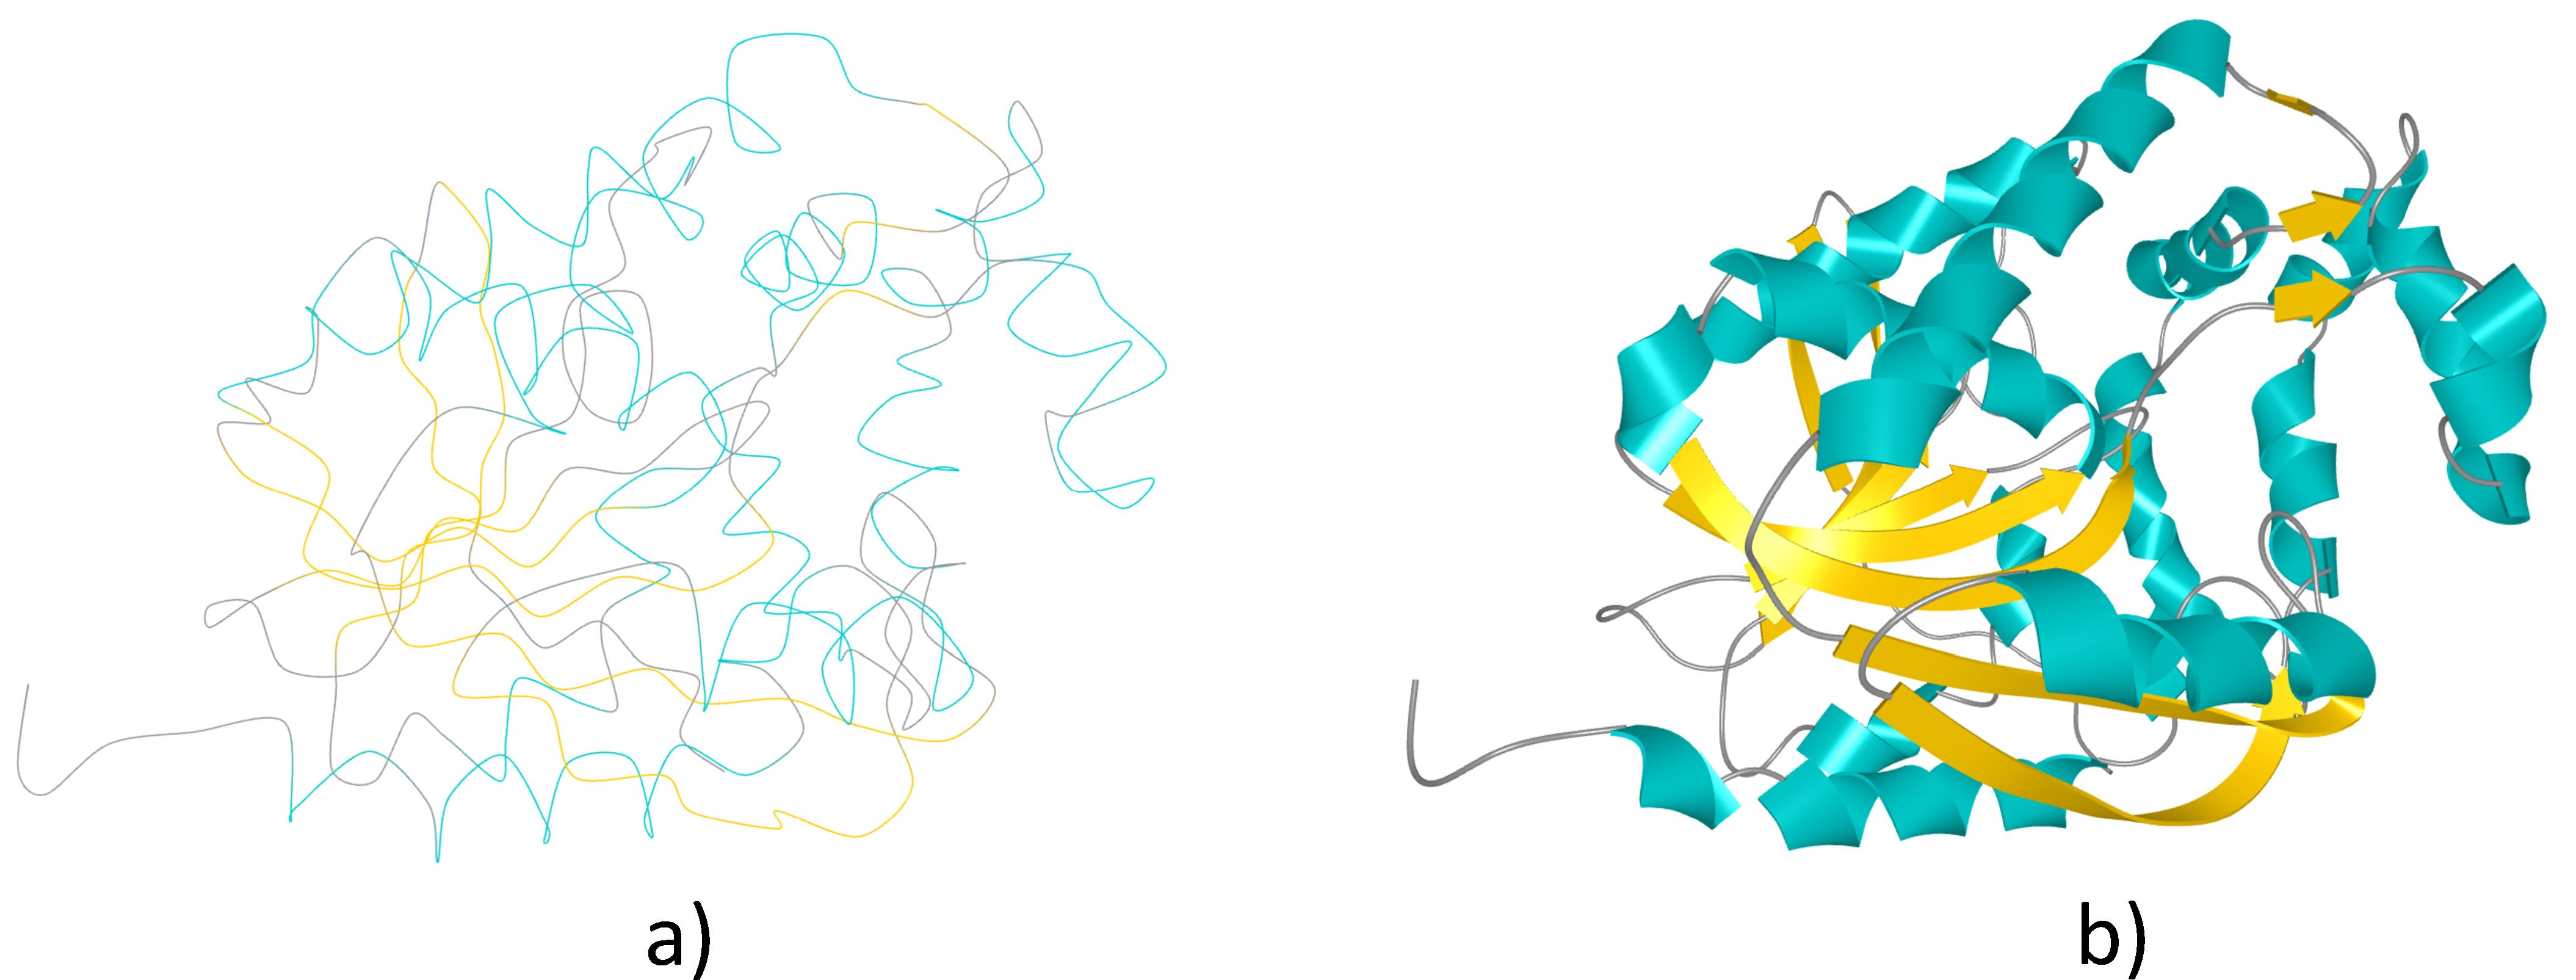
\includegraphics[width=\linewidth]{pictures/representations.pdf} 
  \caption{Types of molecular representations in modern visualization tools: a) alpha trace b) ribbon diagrams}
  \label{Fig:vis2}  
\end{figure} 

In 1981 Jane S. Richardson published \textit{cartoon} illustrations of all then known protein structures \cite{richardson1981anatomy}. In these schematic representations, known today as \textit{ribbon diagrams}, she used consistent and intuitive illustrations of secondary structures to demarcate their position along protein backbone. Although ribbon diagrams were originally hand drawn, they are nowadays part of every molecular visualization software (Figure \ref{Fig:vis2} b)).

Currently the fastes approaches to visualization of ribbon diagrams include the two stage approach by Wahle and Birmanns \cite{wahle2011gpu} where first the backbone tube is generated on CPU and than the vertices are adjusted on GPU to form the final geometry. Another adaptive method by Hermosilla et al. \cite{hermosilla2015instant} takes advantage of the tessellation shader and generates only the geometry needed for current viewpoint.

\subsection{Surface Representations}
\label{Sec:surfaces}
These representations communicate the internal structure of the protein. However in many cases the focus of interest is on the surface of the protein, since the surface is the part of protein that is in contact with outer environment. It is therefore important for biochemists to identify the boundaries of the proteins that are accessible to ligands or interacting with other proteins.

We have already mentioned one type of surface defined by atom spheres of van der Walls radii and therefore called \textit{van der Waals (vdW) surface} \cite{richards1977areas} -- Figure~\ref{Fig:surface} (blue). This surface indicates the precise molecular volume (Figure \ref{Fig:simple} a)).

Another type of surface -- \textit{solvent accesible surface (SAS)} was developed to show the regions of molecule accesible by a solvent molecules \cite{lee1971interpretation}. Here, the solvent molecule is approximated by a spherical probe, which rolls rolls over the vdW surface. The center of the probe than defines the SAS surface -- Figure~\ref{Fig:surface} (yellow). In other words, solvent accesible surface is equal to a vdW surface inflated by the radius of probe.

\begin{wrapfigure}{l}{0.5\textwidth} 
\vspace{-20pt}
\begin{center}
  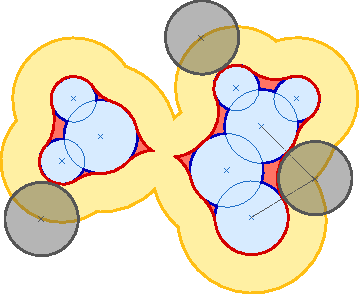
\includegraphics[width=\linewidth]{pictures/surface.pdf} 
  \caption{Schematic representation of molecular surfaces: vdW surface (blue), SES (red) and SAS (yellow). The SES and SAS are defined a probe (grey) rolling over vdW surface. Image taken from \cite{kozlikova2015visualization}.}
  \label{Fig:surface}  
\end{center}
\vspace{-20pt}
\end{wrapfigure}

\textit{Solvent excluded surface (SES)} \cite{richards1977areas} is defined in similar manner to SAS. However, instead of the center of the probe, its outer shell defines the surface -- Figure~\ref{Fig:surface} (red). It was the first smooth surface defined and thanks to the close approximation of molecular volume it is one of the most used surface representations (Figure \ref{Fig:simple} b)). Many algorithms for its computation and visualization have been developed over the years. Currently the fastest soulutions include paralelization of contour-buildap algorithm \cite{totrov1996contour} -- algorithm that computes track of the probe on atom surfaces -- by Lindow et al. \cite{lindow2010accelerated} and Krone et al. \cite{6094043} as well as a grid-based approach by Hermosilla at al. \cite{hermosilla2017interactive} that utilizes progressive surface refinement for rendering of dynamic models on the fly.

\textit{Ligand exluded surface (LES)} is a relatively new generalization of SES proposed by Lindow et al. \cite{lindow2014ligand}. Instead of using an approximate probe, it uses full geometry of ligand to generate the surface. It thus illustrates the precise accessibility, however it is very computationally demanding (Figure \ref{Fig:simple} c)).

Yet another type of molecular surface -- \textit{molecular skin surface (MSS)} was proposed by Edelsbrunner \cite{edelsbrunner1999deformable} (Figure \ref{Fig:simple} c)). The shape of MSS depends on the single parameter \textit{s} -- shrink factor. The advantage of MSS over SES is full $C^1$ continuity.  Among the fastest aproaches to generation of MSS belong the ones by Lindow et al. \cite{lindow2010accelerated} and Yan et al. \cite{Yan2017}.

In 1982 Blinn \cite{blinn1982generalization} proposed use of a Gaussian convolution
kernel to blend atom potentials to achieve an approximation of molecular surface. This technique callled \textit{convolution surface model (CSM)} is more commonly known as Metaballs (Figure \ref{Fig:simple} e)). As with other techniques, improvements and new kernels have been proposed over the years (e.g. by Krone et al. \cite{krone2012fast}) and the resulting techniques belong to the fastest surface rendering approaches. 

\begin{figure}[H]
  \centering
  \includegraphics[width=\linewidth]{pictures/surface2.pdf} 
  \caption{Comparison between different molecular surfaces of the protein isomerase: a) vdW surface b) SES with probe radius 1:4 Å c) LES for equilenine d) MSSwith shrink factor 0.35 e) Gaussian surface with standard deviation equal to the atom radius. Image taken from \cite{kozlikova2015visualization}.}
  \label{Fig:surface2}  
\end{figure}

\subsubsection{Surface Simplification}
With larger kernels, the CMS can be used for simplification of molecular surface, showing just the general shape of the protein. This is sometimes required, as molecular surfaces are often used for mapping of other properties of proteins and atomistic models with many occlusions and high visual complexity are not suitable for this purpose.

Couple of other approaches for surface simplification have been proposed. \textit{Coarse graining} \cite{levitt1976simplified} is method that groups several atoms (e.g. one amino acids) together. These groups are than represented by single sphere. Another approach is mapping the molecular surface to spherical coordinates \cite{postarnakevich2009global}.

\begin{wrapfigure}{l}{0.5\textwidth} 
\vspace{-10pt}
  \begin{center}
  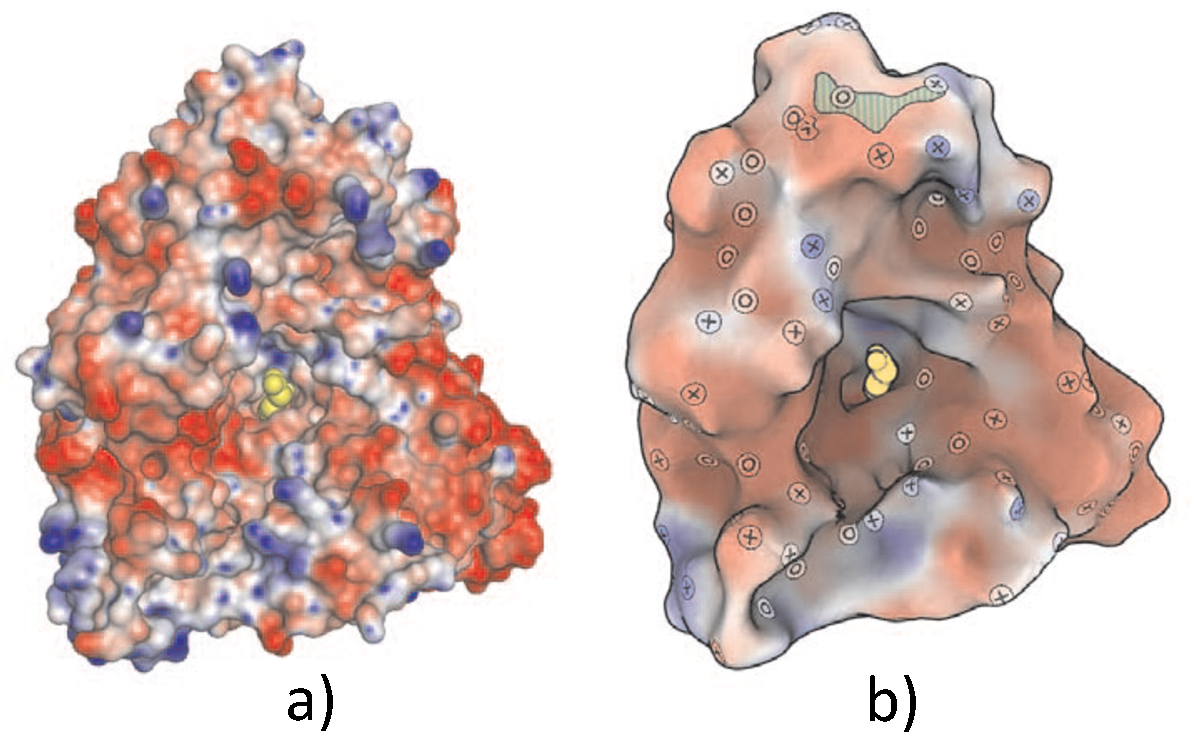
\includegraphics[width=0.95\linewidth]{pictures/simpl.pdf} 
  \caption{Simplified surface representation proposed by Cipriano and Gleicher. a) SES b) simplified surface. Image taken from \cite{cipriano2007molecular}.}
  \label{Fig:simple}  
	\end{center}
  \vspace{-30pt}
\end{wrapfigure}

Cipriano and Gleicher \cite{cipriano2007molecular} proposed a method that uses a combination of
filters and mesh restructuring to smooth the low frequency parts of the surface and generate a simplified representation of overall shape of the protein (see Figure \ref{Fig:simple}). Markings are then placed on the surface to indicate the important removed details as well as other features of the surface, such as the physico-chemical properties of surface amino acids.

\subsubsection{Visual Enhancements}
Another way of dealing with high visual complexity of molecular structures is introduction various visual enhancements. One the most employed visual cues in molecular rendering is certainly \textit{ambient occlusion (AO)} \cite{miller1994efficient}. The goal of this technique is to calculate, how each object in the scene is exposed to the ambient lighting. It is computationaly very expensive, however the latest results from Hermosilla et al. \cite{hermosilla2016high} enable real time rendering of AO for MD simulations.

In their work, they also cover rendering of another common effect -- \textit{halos}. Haloes are highlights extending from selected object boundaries (used e.g. to indicate ligand in an MD simulation). Similar to them are also \textit{depth-dependent silhouettes}, that contour the edges  detected from scene depth map. Another effect for guidance of attention was adapted from photography -- \textit{Depth of Field} simulation blurs the objects that are out of focus. 
Other rendering techniques, such as \textit{toon shading}, \textit{line drawing} and \textit{hatching} are commonly used for molecular rendering as well, since they can be adjusted to emphasize important features \cite{kozlikova2015visualization}.

%\subsection{Molecular Visualization Systems}

\section{Analysis of Protein Voids}
We have described many possible representations that support the analysis of proteins in general. In this section, we will focus on one of the most important features of proteins -- their inner voids. As we mentioned before, the active site -- the reactive area of the protein is often buried deeply inside of the protein structure and accessible only via those voids, namely tunnels. Therefore, the extraction and analysis of these tunnels is vital for the study of protein-ligand binding. Here, we will mention only several most videly used principles of the approaches used in this area, as the extensiveness of this work exceeds the capacity of this thesis. Complete overview of the published tools for detection and analysis of biomolecular cavities can be found in state of the art reports by Krone et al. \cite{krone2016visual} and Simões et al. \cite{simoesgeometric}.

\subsection{Detection of Protein Voids}
There are several methods for extracting the shape of the protein voids in general, as well as numerous ones focusing on tunnels specifically. The algorithms can be classified into several categories, depending on the approach they use: grid-based, probe-based, Voronoi-based, surface-based, path analysis and ligand based. Most of the algorithms combine several approaches, in order to achieve better results. Moreover, we can differentiate  between algorithms applicable only for static structures and algorithms taking into account molecular dynamics.

Many algorithms for void detection use a voxel grid to subdivide the 3D space containing the protein. The basic ide of purely \textit{grid-based approaches} is to split voxels into two groups -- those that lie inside a protein atoms and those that lie in a void space. 
The grid points from the second group are then assigned value based on different properties -- distance to the protein atoms (\cite{levitt1992pocket, Petrek2006Caver, hendlich1997ligsite}), interaction energies (\cite{an2005pocketome, laurie2005q, hernandez2009sitehound}) or protein and solvent 
\begin{wrapfigure}{r}{0.5\textwidth}
\vspace{-17pt}
  \begin{center}
  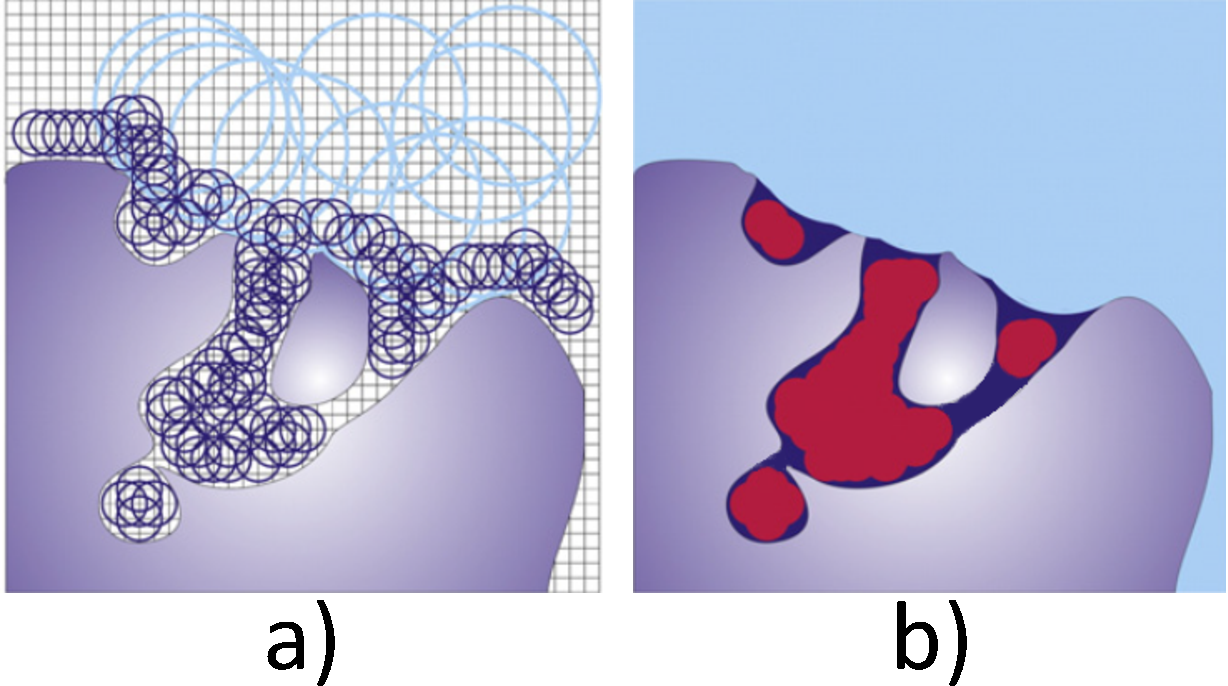
\includegraphics[width=\linewidth]{pictures/rollingprobe.pdf} 
  \caption{Rolling probe method. a) Two kinds of probes are placed in each point of the grid. b) The identified volumes are divided into the protein surrounding (light blue), and internal voids (red). Dark blue areas indicate undetected internal volume. Image adapted from \cite{brezovsky2013software}.}
  \label{Fig:rollingprobe}  
	\end{center}
  \vspace{-25pt}
\end{wrapfigure}
residence probability extracted from MD simulation (\cite{raunest2011dxtuber, krone2011interactive, kokh2013trapp, paramo2014efficient}). The evaluated grid is further processed to extract the cavities using e.g. flood-fill segmentation or path analysis to find the cheapest path from active site to the surface of the protein.
%An exaple of a \textit{grid-based approach} that also utilizes \textit{path analysis} is the first version of CAVER algorithm \cite{Petrek2006Caver}. Here, each node of the grid is assigned a cost, based on the maximal radius of a hypothetical ball that can be inserted into a node without intersecting voxels occupied by protein atoms -- the larger the radius, the lower the cost. A graph searching algorithm than searches for cheapest path leading from user defined active site to the outer boundary of protein. This path is than taken as tunnel centreline and the detected tunnel is tan represented as a set of maximal spheres placed on centreline.

Second group of algorithms utilizes \textit{grid-based approaches} in combination with  \textit{probe-based approaches}. For example, HOLLOW \cite{Ho2008Hollow} and 3V \cite{voss20103v} algorithms use two probe spheres of different sizes that are placed in each node of the grid (see Figure \ref{Fig:rollingprobe}). The probes that do not intersect with protein atoms define the surface of the protein -- large probe defines the outer surface, while the smaller one defines also the inner voids. This approach is also referred to as \textit{rolling probe} principle. Different combinations probe-based and grid-based approaches can be found e.g. in \cite{kleywegt1994detection, czirjak2015princces, laskowski1995surfnet, yu2009roll}.

\begin{wrapfigure}{l}{0.6\textwidth}
\vspace{-17pt}
   \begin{center}
  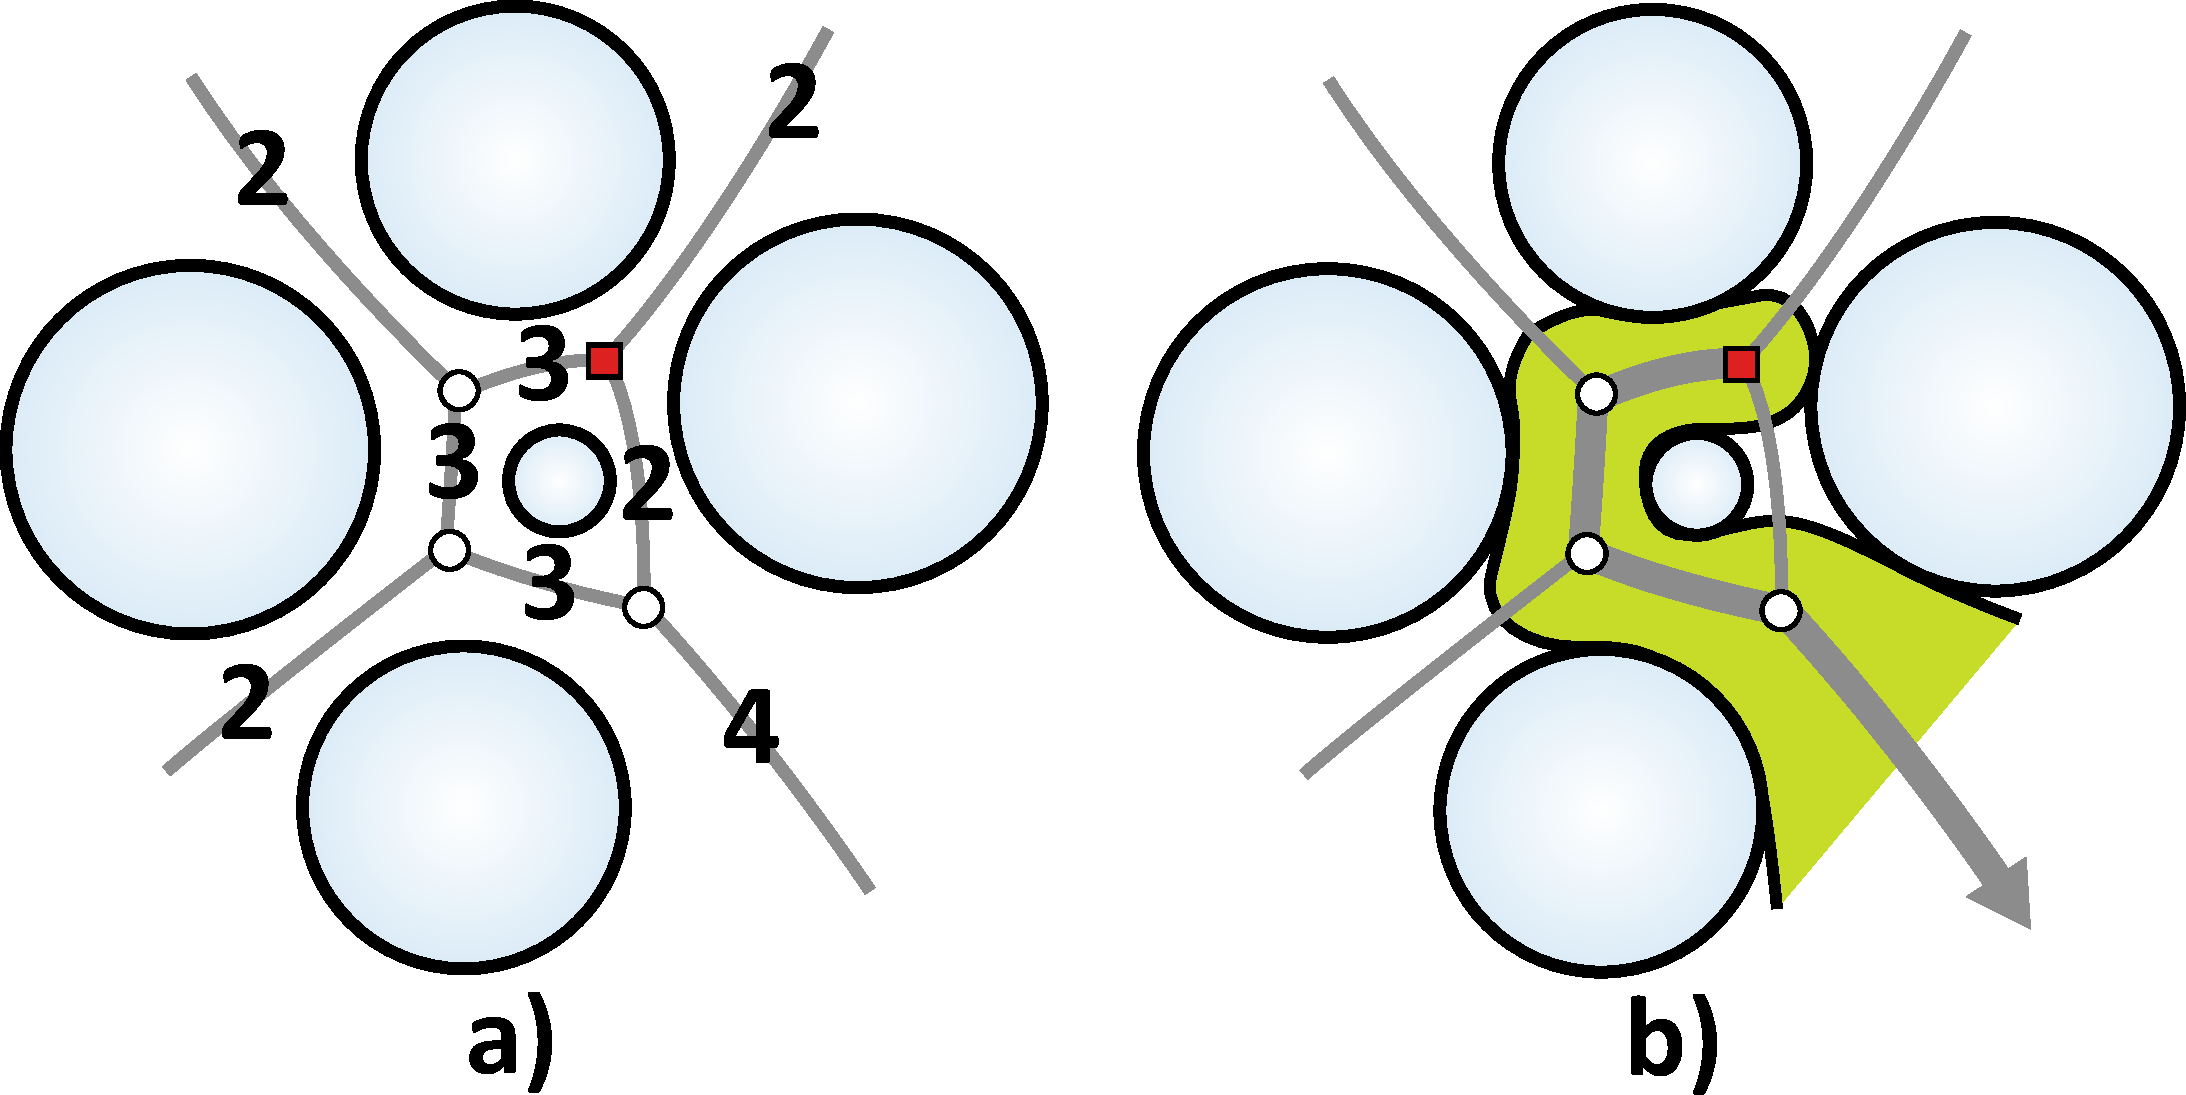
\includegraphics[width=\linewidth]{pictures/voronoi.pdf} 
  \caption{Example of Voronoi-based tunnel detection. a) Evaluated edges. b) Path with highest score found by Dijkstra's algorithm. Red square indicates active site. Image adapted from~ \cite{caver20}}
  \label{Fig:voronoi} 
   \end{center} 
   \vspace{-17pt}
\end{wrapfigure} 

Accuracy of grid-based algorithms strongly depends on the resolution of the voxel grid. At the same time, high resolution of the grid leads to high memory demands of these algorithms. \textit{Voronoi-based} algorithms in combination with \textit{path analysis} address these drawbacks by utilizing Voronoi diagrams to subdivide the 3D space of protein structure (see Figure \ref{Fig:voronoi}). Each atom of the protein forms a center of Voronoi cell. The edges are then evaluated by cost function, which assigns the value based on distance of the edge from the cell centres (i.e. atom centres). Then, Dijkstra's algorithm is used on the edge graph to find the best path from the active site towards protein surface. This principle is used and improved upon in \cite{Petrek2007MOLE, caver20, Yaffe2008MolAxis}. Chovancova et al.~\cite{caver30} extend this approach for detection of tunnels taking into account the movement of the protein in CAVER 3.0 algorithm. It computes tunnel paths for each time frame of MD simulation. Than the corresponding paths are clustered. Thus it is possible to track the evolution of the tunnels in time.

Another set of void detection methods is based on theory of $\alpha$-shapes. First, they compute Voronoi diagram on the atoms of the protein in a same manner as previous methods and transform it to Delaunay triangulation. Than, all the triangles that do not lie completely inside the protein atoms are deleted, resulting in an $\alpha$-shape of the protein. The cavities can than be easily extracted from the $\alpha$-shape. This method was first used in CAST~\cite{liang1998anatomy} and was later extended and generalized by \cite{sridharamurthy2016extraction, kim2013tunnels, masood2015chexvis}.

In Section \ref{Sec:surfaces} we have described several methods for extraction of molecular surfaces. Based on these methods, several \textit{surface-based} approaches for detection of cavities have been proposed. For example, Jurčík et al. \cite{jurvcik2016accelerated} extend the method proposed for computation of SES by Krone et al.~\cite{6094043} to detect also closed cavities. Coleman and Sharp \cite{Coleman2009CHUNNEL} use triangulation of SES to detect channels in proteins. Krone et al. \cite{krone2013interactive, krone2014visual} proposed a method for real time GPU accelerated extraction of cavities based on Ambient Occlusion. The LES method proposed by Lindow et al. \cite{lindow2014ligand} enables extraction of cavities based on the actual geometry of the ligand.

The tunnel detection can be alternatively viewed as a path planning problem -- the task is to find a collision free path for ligand starting at active site and leading to the surface. Path planning approaches to tunnel detection usually employ Rapidly Exploring Random Trees \cite{lavalle1998rapidly} (RRT), a technique that builds a tree of collision free configurations moving through the defined space. This approach can be applied directly on an MD simulation, thus it avoids the computationally expensive step of traditional, e.g. Voronoi-based approaches, where correspondence between geometry computed in different MD snapshots has to be found. Most notable work in this are includes \cite{cortes2005path, vonasek2016application, vonasek2017tunnel}.

\subsection{Visual Analysis of Protein Tunnels}


ligand md simulations

\section{Protein-Protein Interactions}

\subsection{Docking}
\subsection{Visual Analysis}
